\documentclass[spanish,notitlepage,letterpaper,12pt]{article} % para articulo en castellano
\usepackage[utf8]{inputenc} 
\usepackage[T1]{fontenc}
\usepackage[spanish]{babel}    % silabea palabras castellanas
\usepackage{subfigure}
\usepackage{amsmath}
\usepackage{amsfonts}
\usepackage{amssymb}
\usepackage[colorlinks=true,urlcolor=blue,linkcolor=blue, citecolor=blue]{hyperref} % navega por el doc
\usepackage{graphicx}
\usepackage{geometry}           % See geometry.pdf to learn the layout options.
\geometry{letterpaper}          % ... or a4paper or a5paper or ... 
\setlength{\topmargin}{0.1in}
\setlength{\textheight}{8in}
\setlength{\textwidth}{6.5in}
\setlength{\oddsidemargin}{0.1in}

\begin{document}

\begin{titlepage}
\begin{center}

{\LARGE{\bf{DETECTOR CHERENKOV}}} \vspace{2mm} \\
{\large{\bf{EN LA UNIVERSIDAD DE LOS ANDES}}}
\vfill
{\large
\begin{tabular}{rl}
{\sc } & {\sc Carlos Guada}
\vspace{1mm} \\
{\sc } & {\sc Yunior Pérez}
\end{tabular}}
\vfill
{\sc LAGO-ULA} \\

\vspace{10mm}
{\Large 2013} 
\end{center}
\end{titlepage}

\tableofcontents

\newpage
\pagestyle{plain}
\setcounter{page}{1}

\section{Detalles Detector}

 \subsection{Ubicación Detector}
El detector se encuentra ubicado en el estado Mérida-Venezuela, zona (sector) la Hechicera,
con una altura de 1893 msn lo que equivale a una profundidad atmosférica 800 g/cm.

      \begin{figure}[htp!]
        \centering
        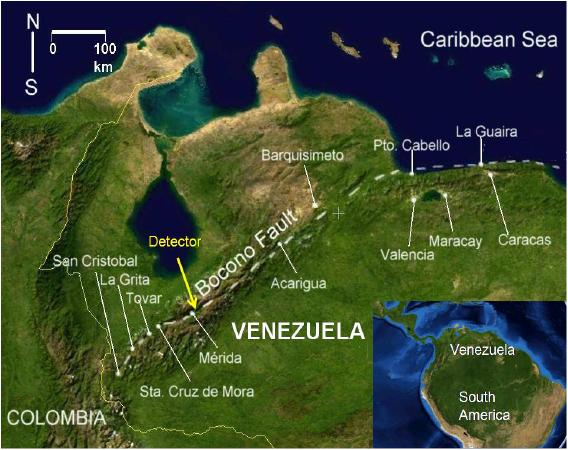
\includegraphics[width=0.50\textwidth,height=0.20\textheight]{imagenes/Ubicaciond.jpg}
        %nexys2.jpeg: 231x218 pixel, 72dpi, 8.15x7.69 cm, bb=0 0 231 218
        \caption{Ubicación geográfica del detector Hugo}
        \end{figure}  

 \subsection{ Tanque de plástico}
 
 Se cuenta con un tanque de plástico de 1 m de Altura y 76 cm de Diámetro.\\
 
   \begin{figure}[htp!]
        \centering
        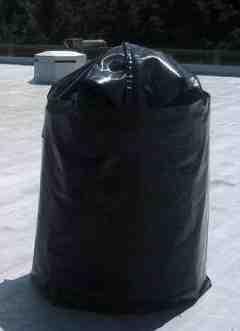
\includegraphics[width=0.30\textwidth,height=0.2\textheight]{imagenes/hugo.jpg}
        %nexys2.jpeg: 231x218 pixel, 72dpi, 8.15x7.69 cm, bb=0 0 231 218
        \caption{Detector Hugo}
        \end{figure}  

 \subsection{Electrónica} 
 
 La electrónica LAGO cuenta con varias interfaces \\
   
     \begin{figure}[htp!]
     \centering
     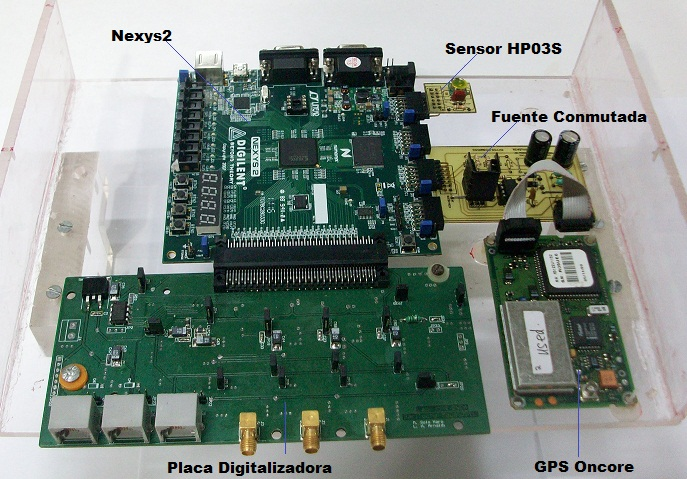
\includegraphics[width=0.65\textwidth,height=0.25\textheight]{imagenes/nuevaLS.jpg}
      % nexys2.jpeg: 231x218 pixel, 72dpi, 8.15x7.69 cm, bb=0 0 231 218
     \caption{Electrónica LAGO}
     \end{figure}  
   
    \begin{itemize}
     \item Nexys2      
     \item Placa Digitalizadora
     \item placa del Sensor HP0S3 
     \item Fuente Conmutada
     \item GPS oncore
    \end{itemize}


    \textbf{ Nexys2}:
     La placa NEXYS-2 es un kit de desarrollo de FPGA de la empresa Digilent, y se utiliza para
     tratar los pulsos digitalizados.
     La alimentación general es de $12V$ (mas de $1 A$) y se conecta directamente a la Nexys2 por algunas de las tres opciones 
     que presenta, dichas opciones son por el cable USB, un conector de batería o conector de alimentación.\,\cite{LAGOOfficial}
 
    \textbf{ Placa Digitalizador}: 
     La placa puede digitalizar simultáneamente hasta tres canales de pulsos. La digitalización se
     realiza con $10bits$ a $40Msps$ \textbf{(Msps = millones de muestras por segundo)} con conversores \textbf{AD9203} de
     Analog Devices.\,\cite{LAGOOfficial}

  \newpage   
  \subsection{Fotomultiplicador} Se cuenta con un fotomultiplicador de 5 pulgadas con su divisor de Voltaje, cuyo diseño fue suministrado
   por la colaboración LAGO- Perú. Este fotomultiplicador esta en procesos de pruebas, lo que se ha obetido hasta ahora es el pulso mostrado
   en figura 7
  
  \begin{figure}[htp!]
     \centering
     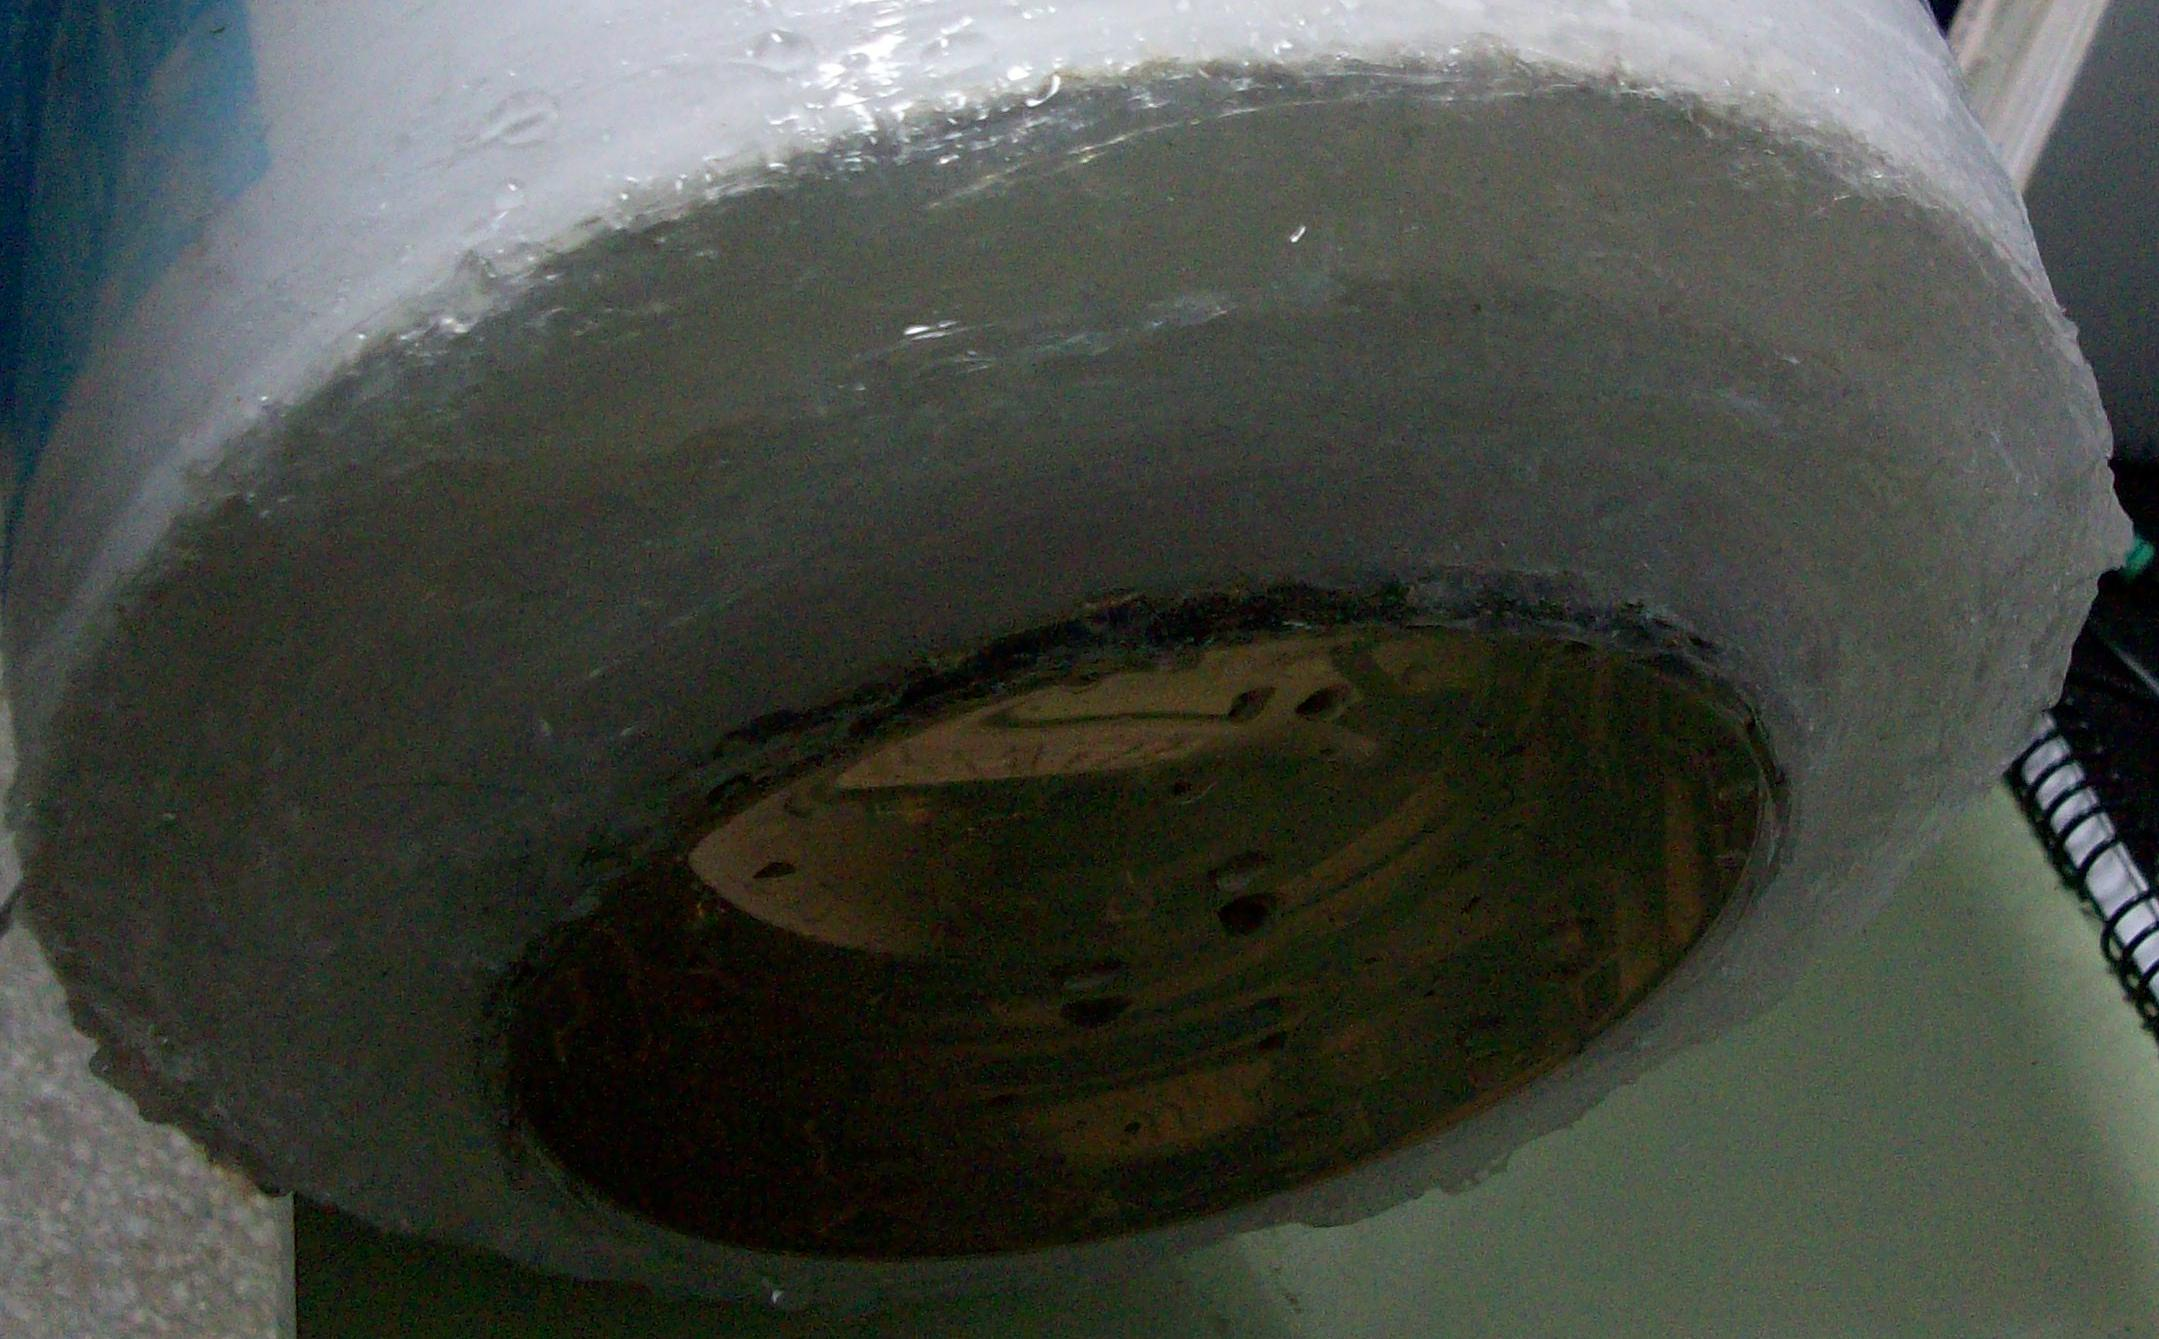
\includegraphics[width=0.20\textwidth,height=0.15\textheight]{imagenes/pmtpeq.jpg}
      % nexys2.jpeg: 231x218 pixel, 72dpi, 8.15x7.69 cm, bb=0 0 231 218
     \caption{Fotomultiplicador de $5^{"}$}
     \end{figure}  
  
  \begin{figure}[htp!]
     \centering
     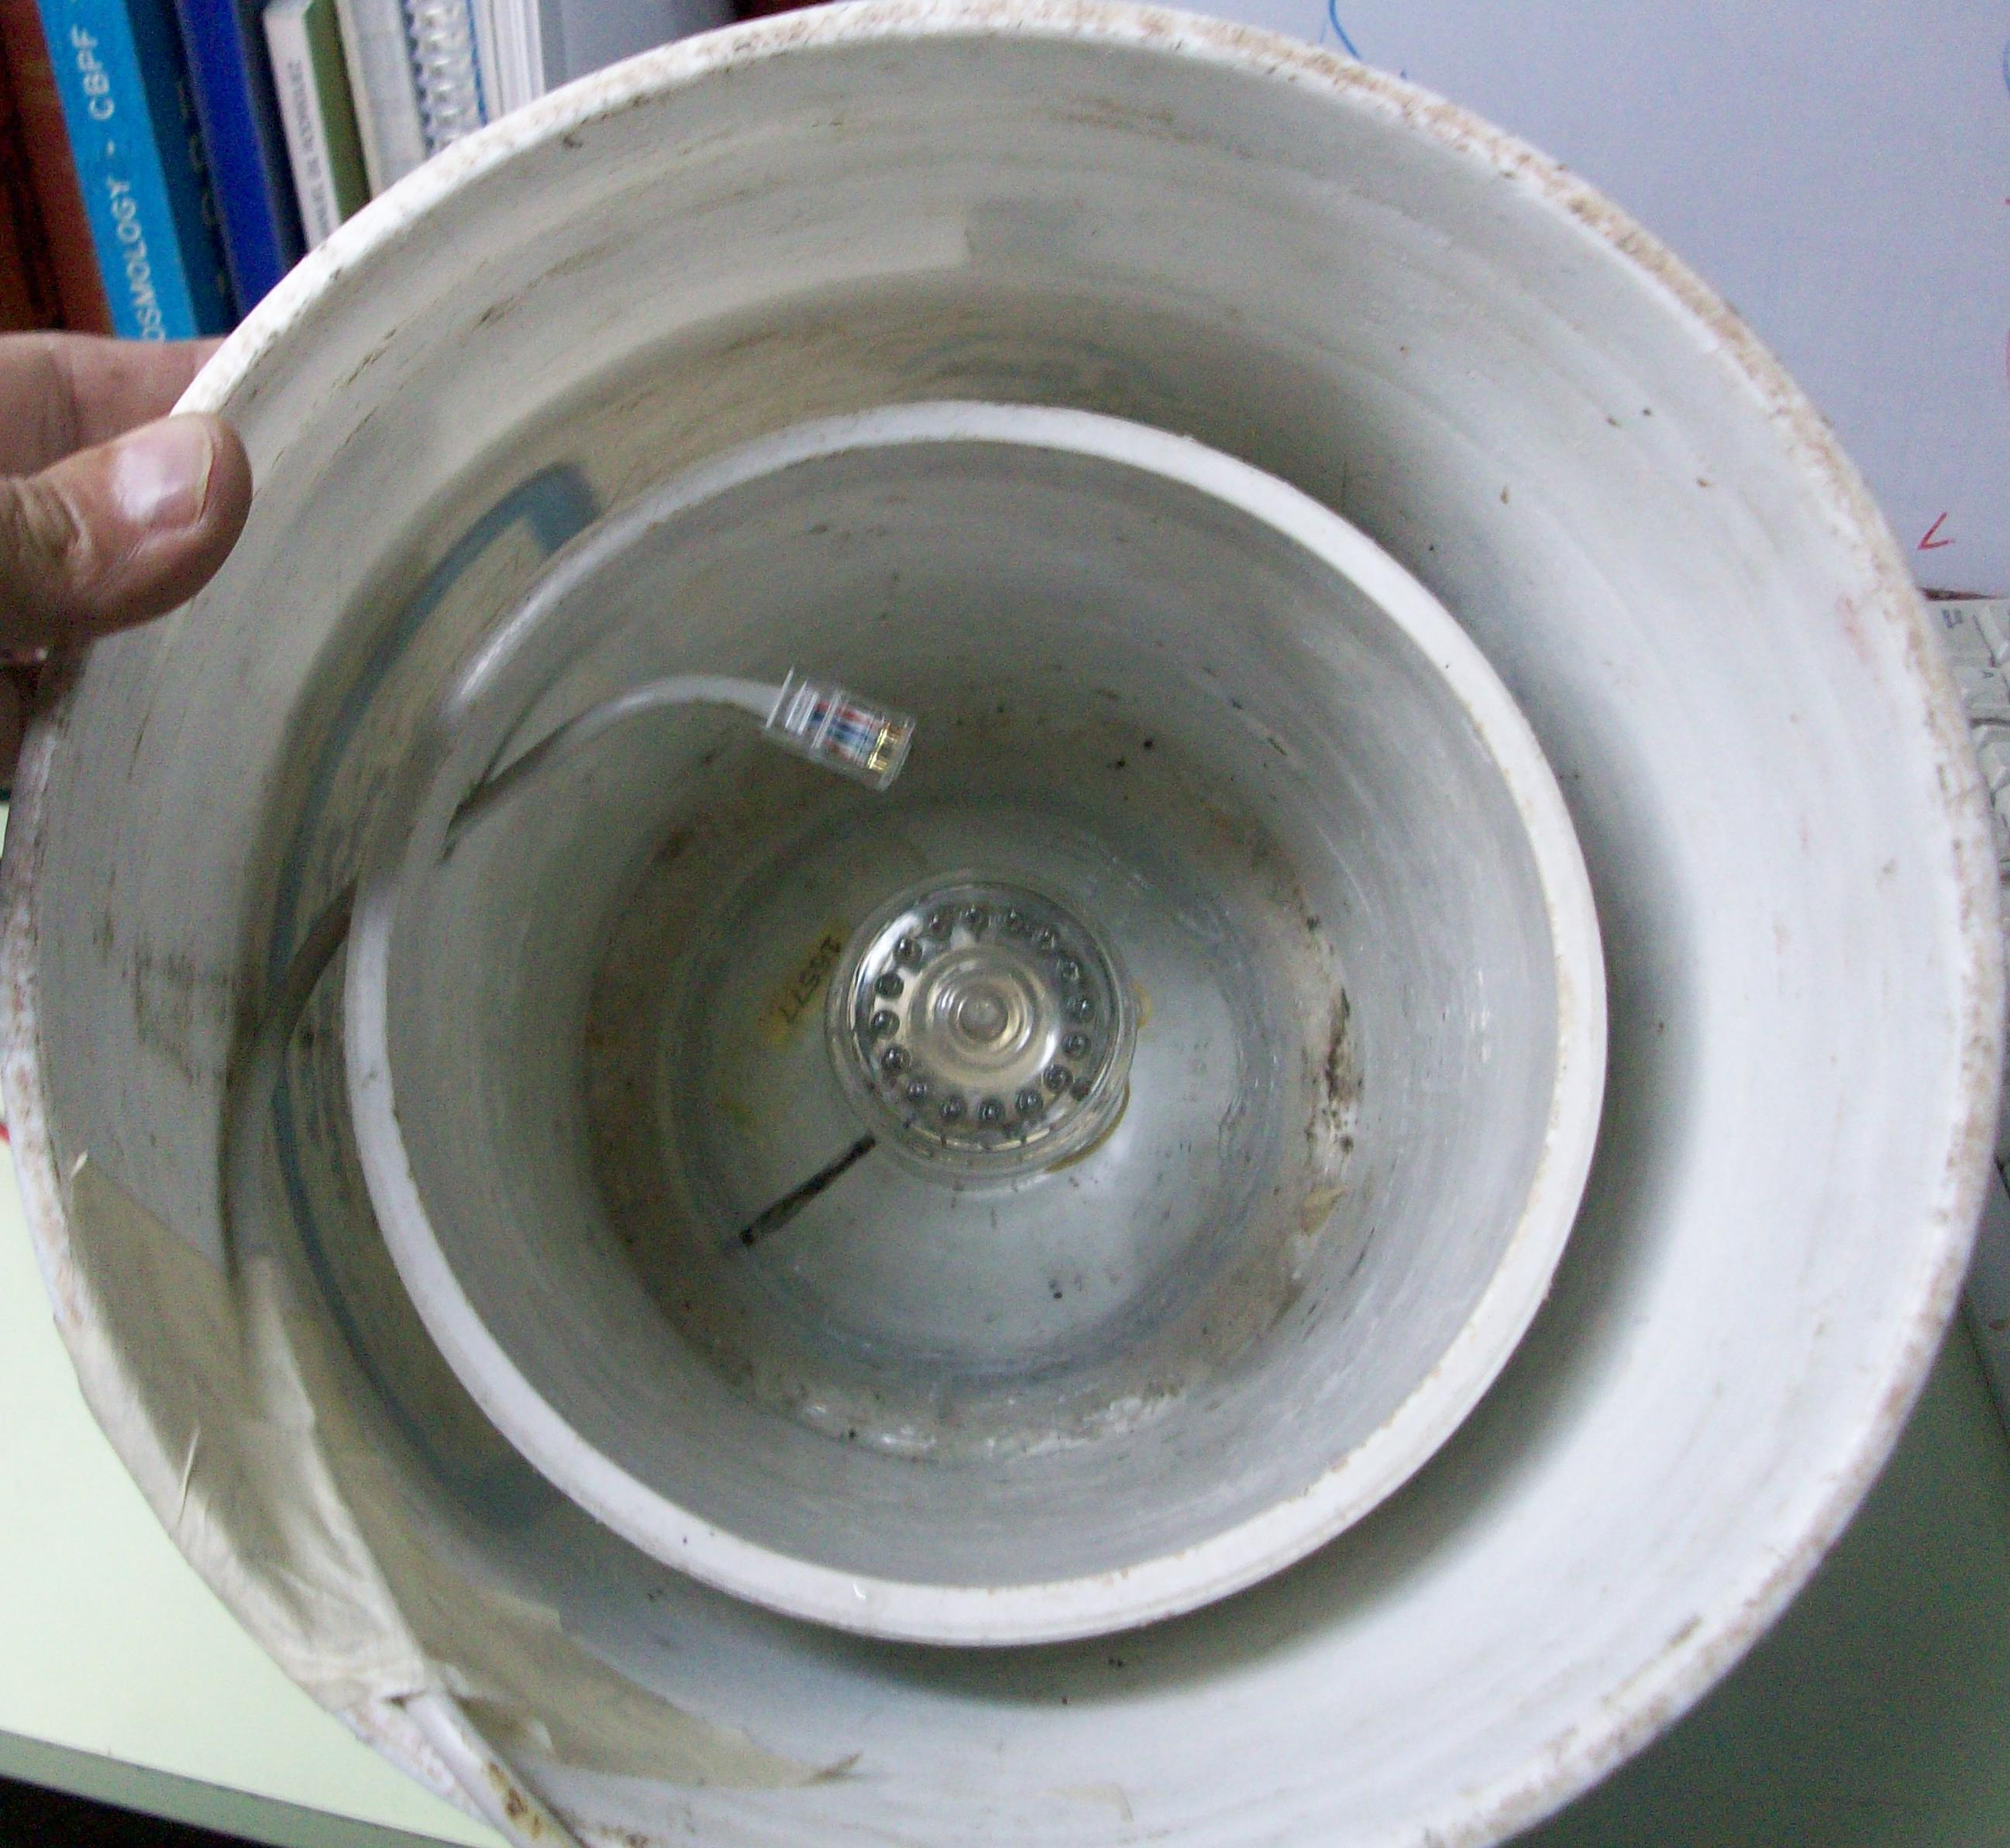
\includegraphics[width=0.20\textwidth,height=0.15\textheight]{imagenes/base.jpg}
      % nexys2.jpeg: 231x218 pixel, 72dpi, 8.15x7.69 cm, bb=0 0 231 218
     \caption{Base fotomultiplicador de $5^{"}$} 
     \end{figure}  
  
   \begin{figure}[htp!]
     \centering
     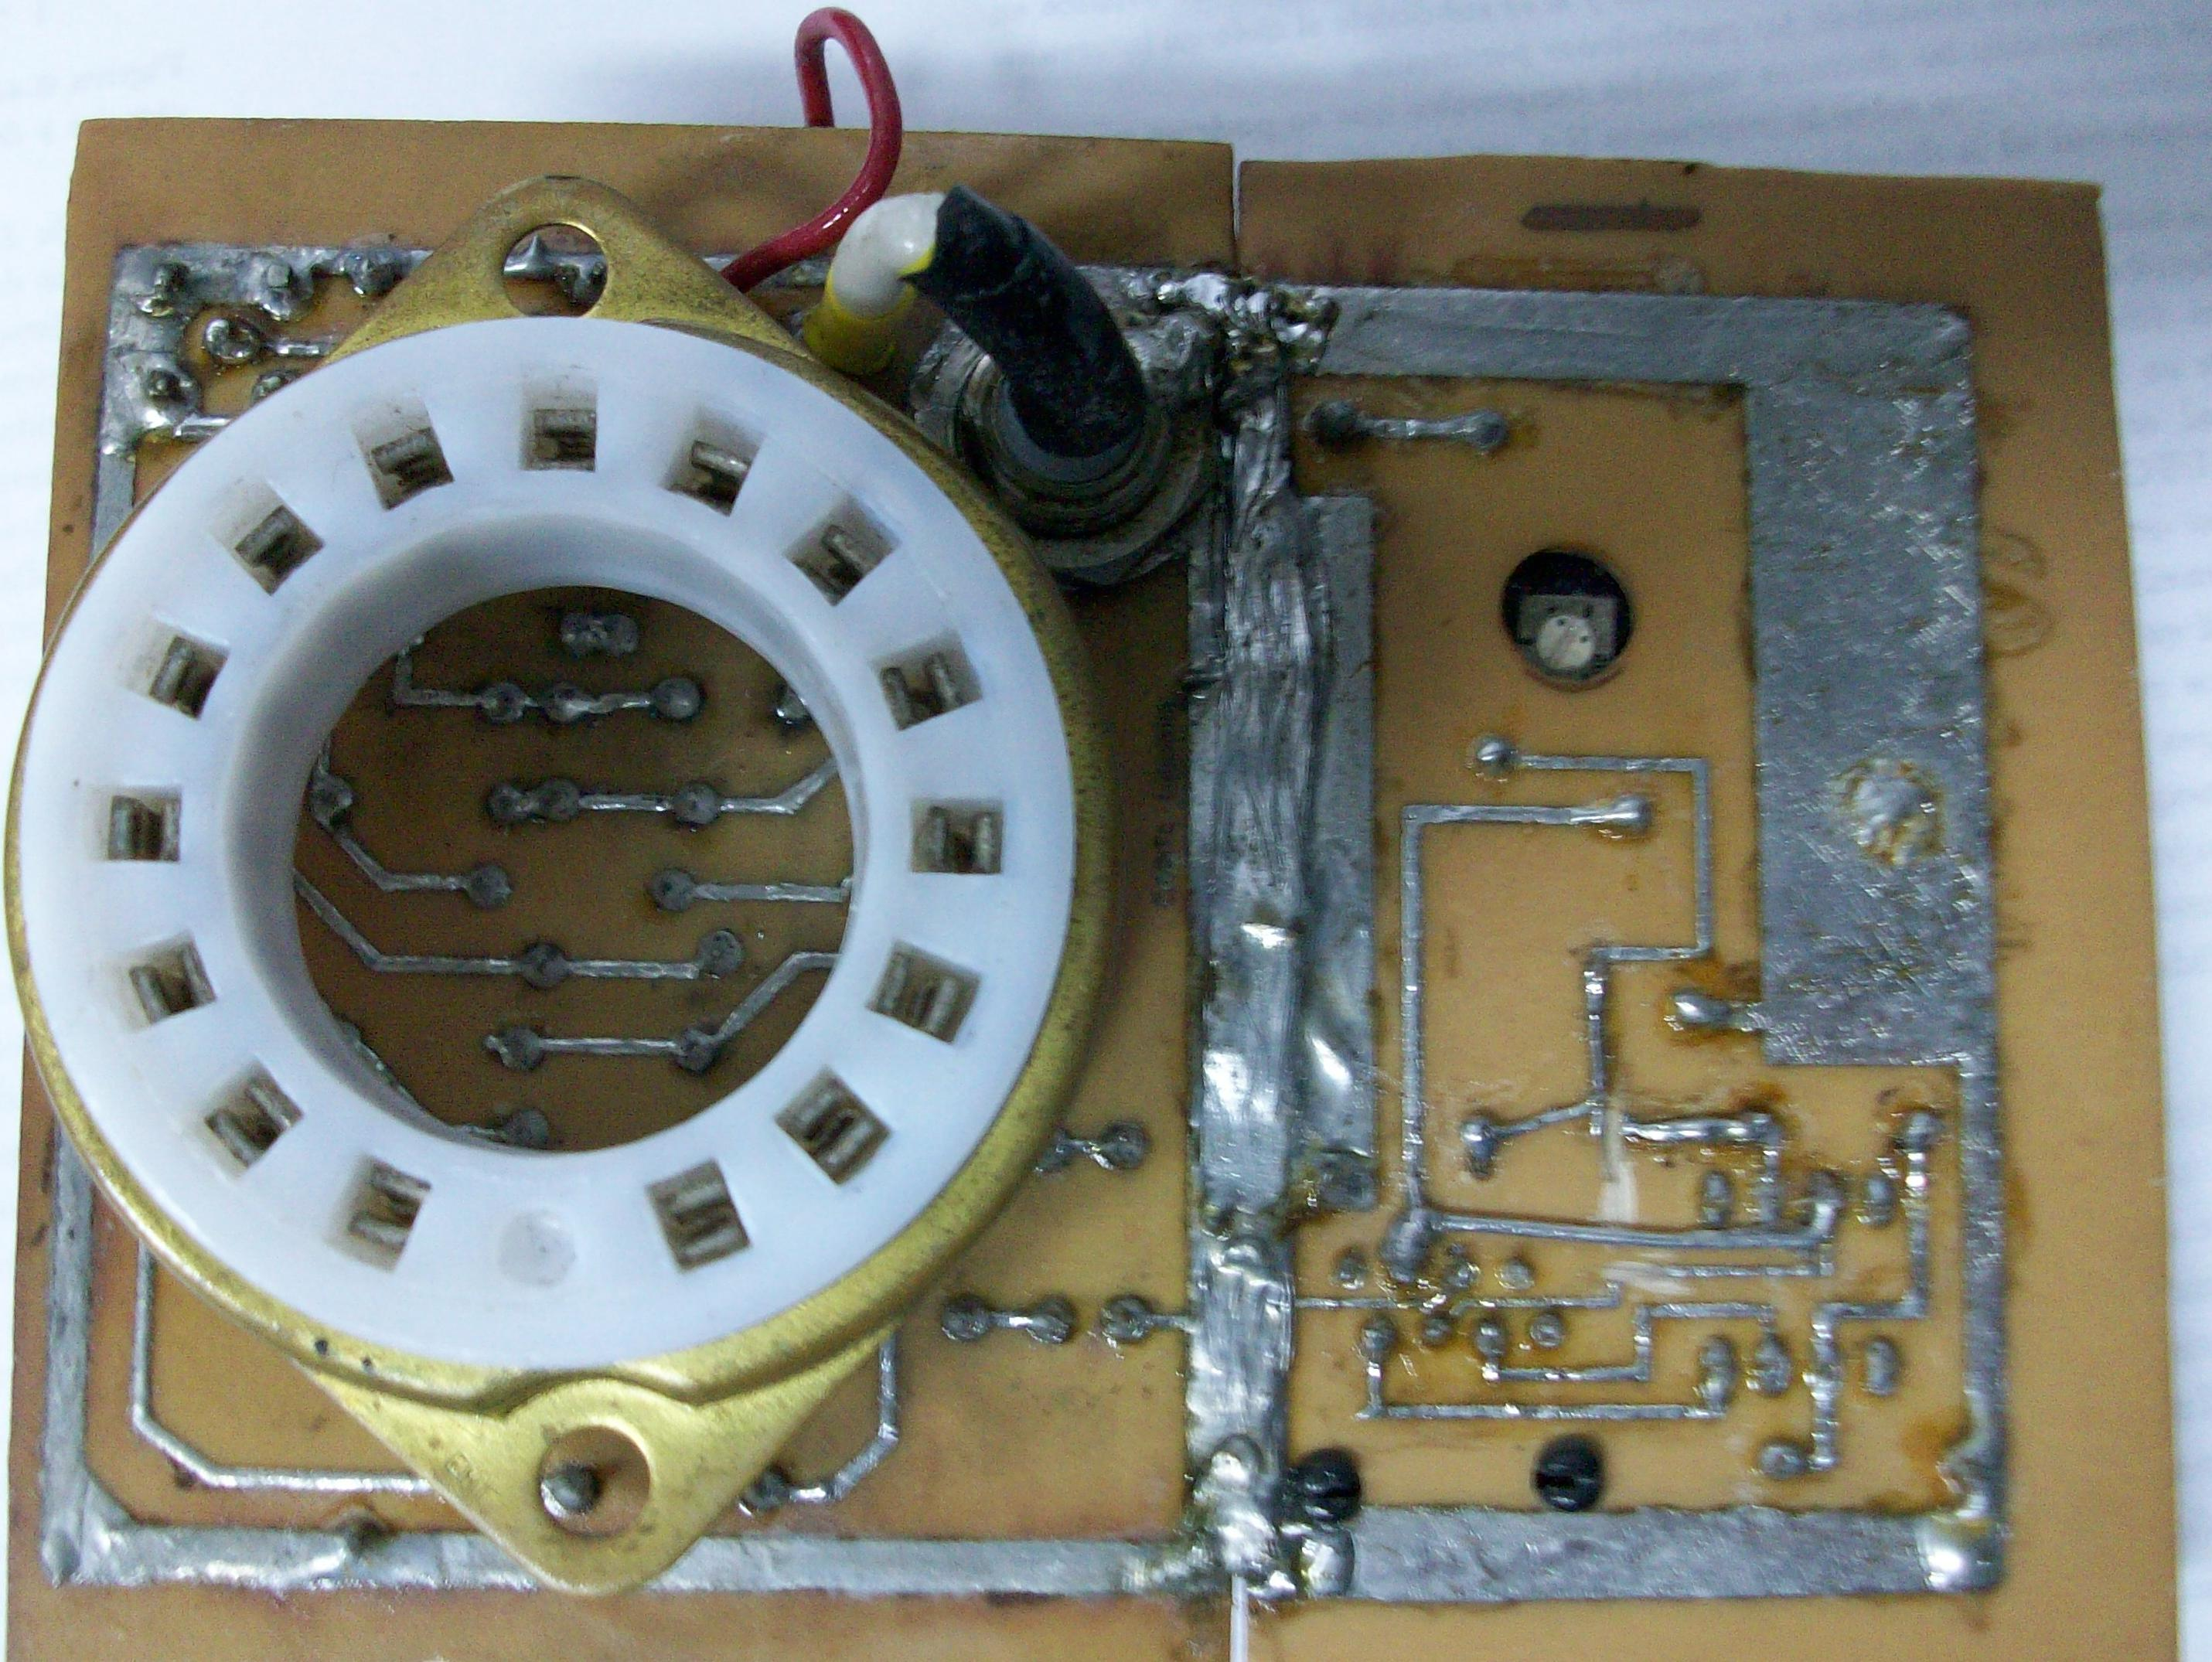
\includegraphics[width=0.20\textwidth,height=0.15\textheight]{imagenes/DivisordeVoltaje.jpg}
      % nexys2.jpeg: 231x218 pixel, 72dpi, 8.15x7.69 cm, bb=0 0 231 218
     \caption{Divisor de Voltaje} 
     \end{figure} 
  
 \subsection{Pulso Obtenido con el Fotomultiplicador Pequeño}  
 \begin{figure}[htp!]
     \centering
     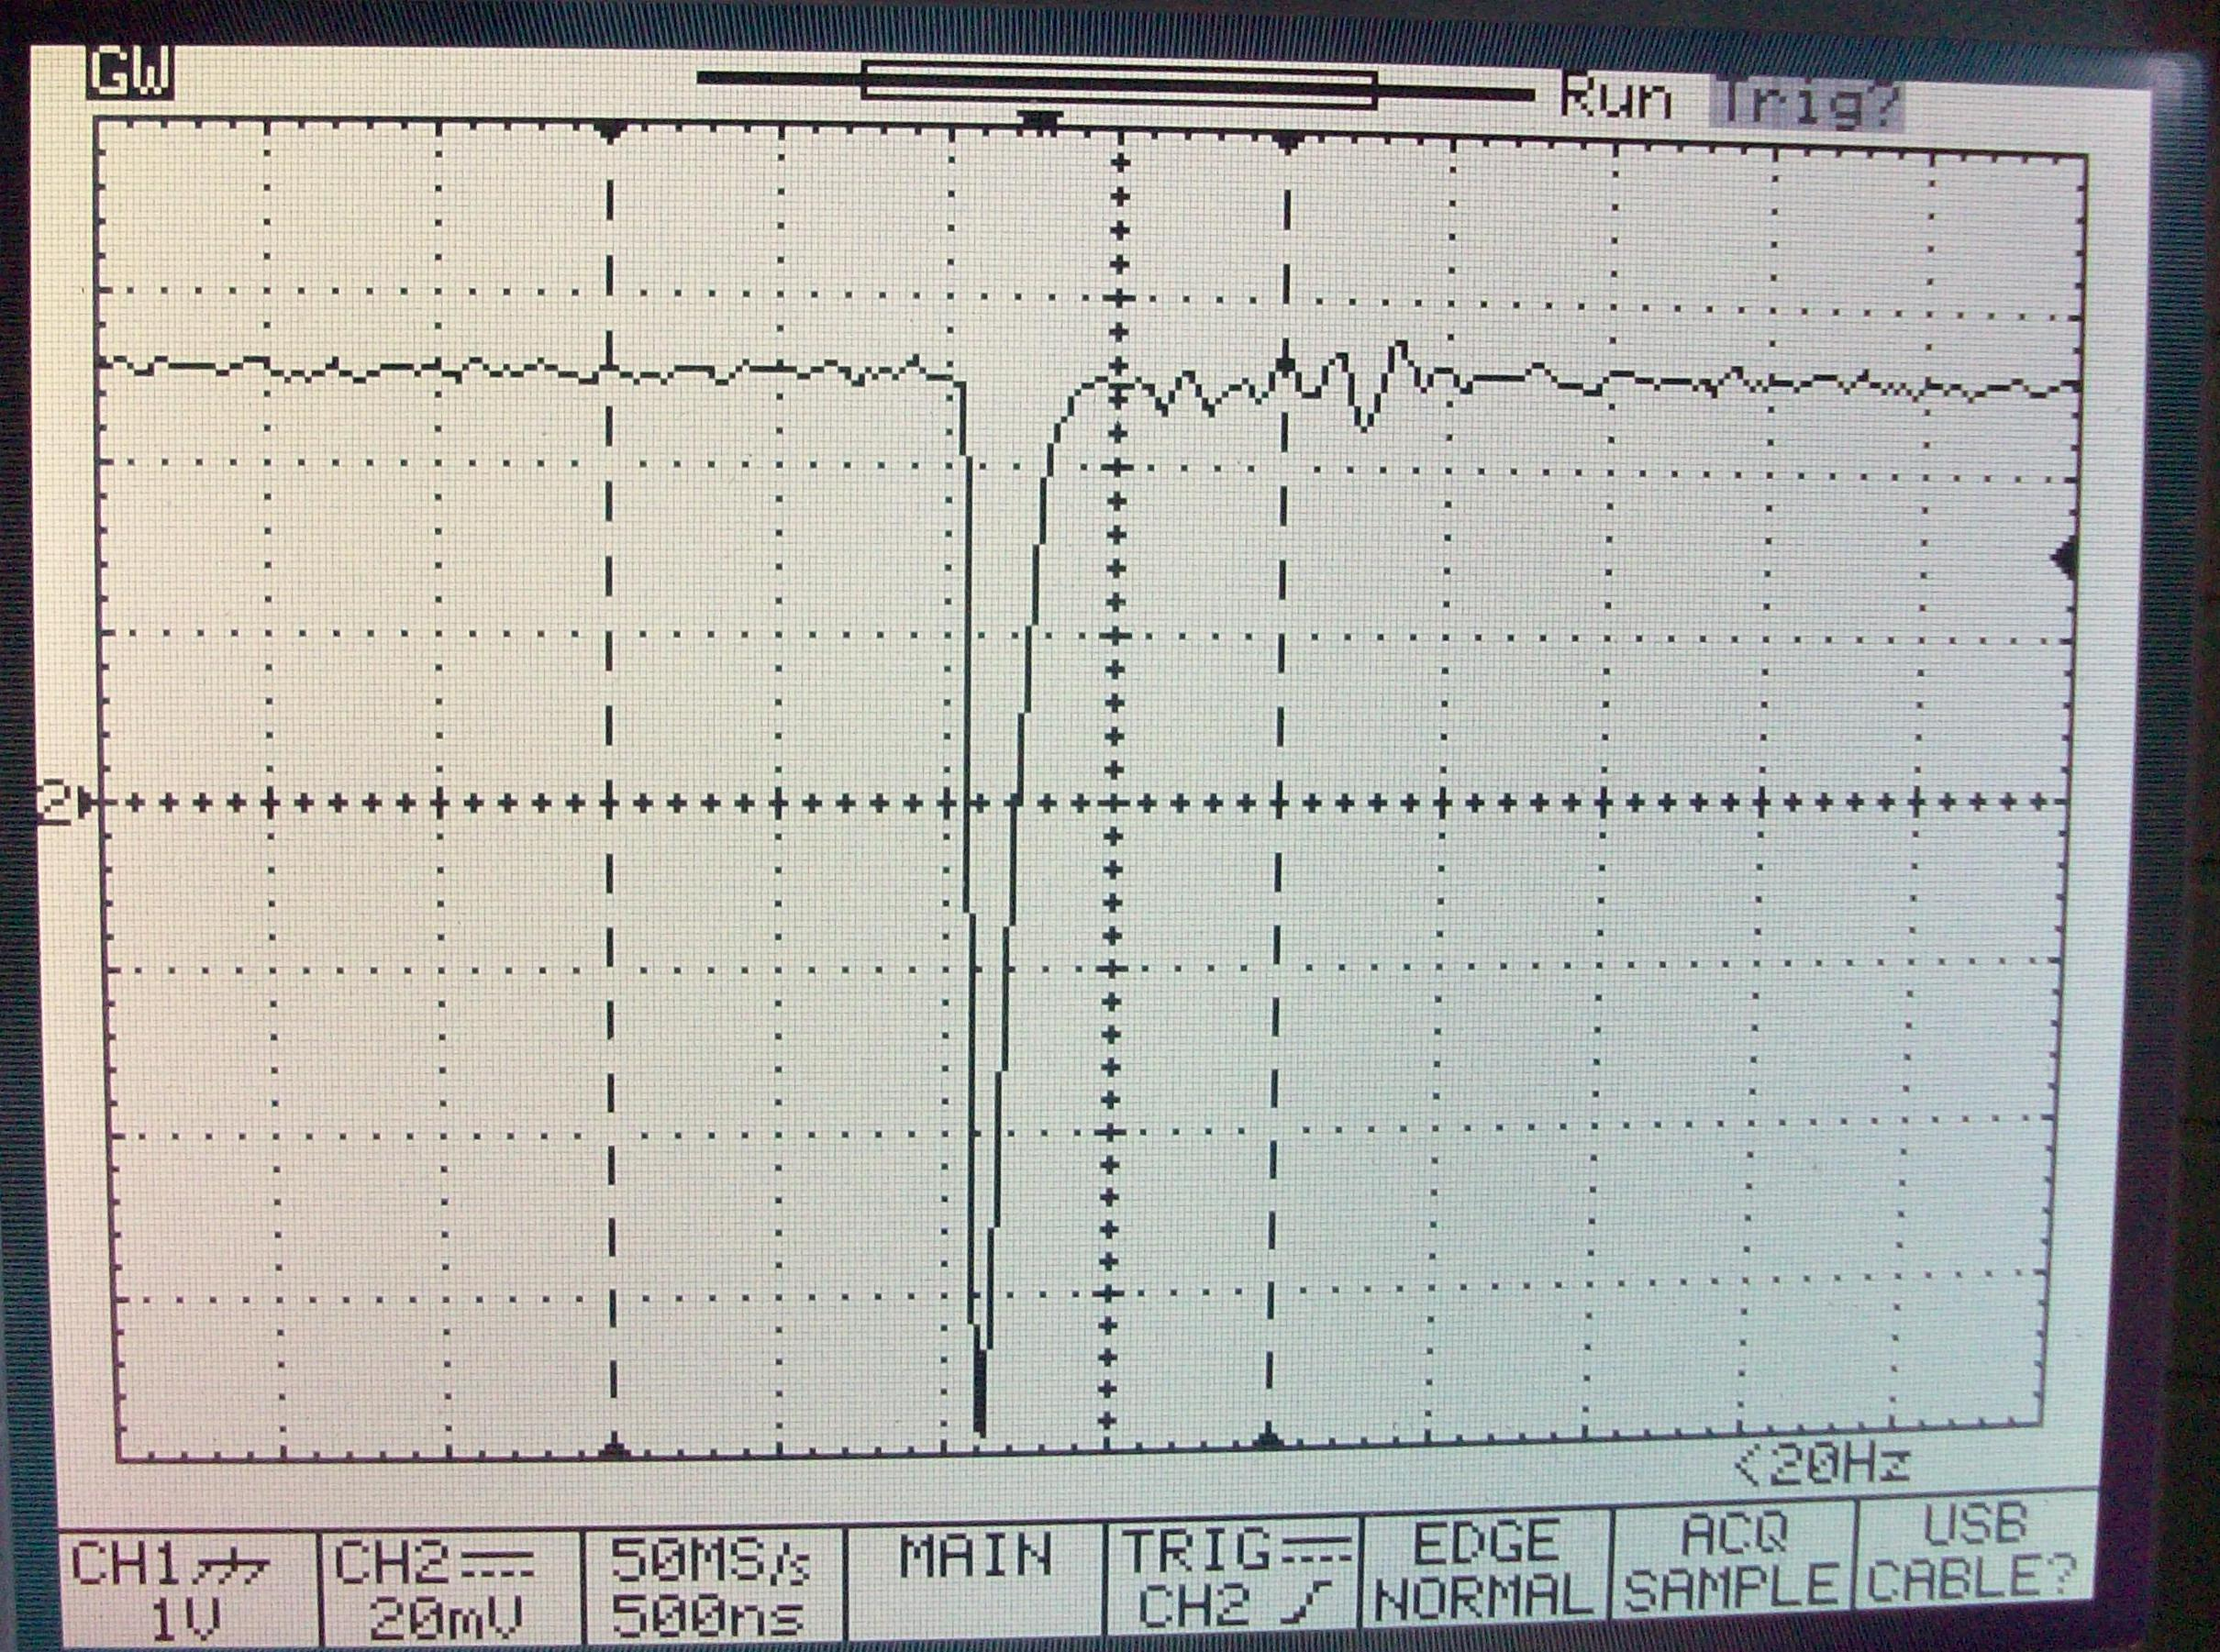
\includegraphics[width=0.65\textwidth,height=0.30\textheight]{imagenes/pulsopmt.jpg}
      % nexys2.jpeg: 231x218 pixel, 72dpi, 8.15x7.69 cm, bb=0 0 231 218
     \caption{Pulso con el Fotomultiplicador Pequeño con un Voltaje de $\sim 1800V$} 
     \end{figure}  
 
  
 \newpage
\section{Bibliograf\'ia}
 
 \begin{enumerate}
  

\bibitem{LAGOOfficial} Miguel Sofo Haro, L. Horacio Arnaldi, H.G. Asorey, M. Gomez Berisso, LAGO Official Electronics guide, 2011.

%  \item Meszaros, P. 2006, de pr\'oxima aparici\'on en Rept. Prog. Phys., e-Print astroph/0605208
%  \item  Atkins, R, et al, 2000, ApJ, 533:L119
%  \item  Pierre Auger Collaboration 2005, 29th International Cosmic Ray Conference, e-Print astro-ph/0604114
%  \item  Allard, D, et al, 2005, 29th International Cosmic Ray Conference
%  \item  Bertou, X,  Allard, D. Nuclear Instruments and Methods. A553: 299-303, 2005
%  \item  Alvarez et al, 2005, 29th International Cosmic Ray Conference
%  \item  LAGO 2006, http://cabtep5.cnea.gov.ar/experiments/lago/
 \end{enumerate}
 
 
\end{document}
